\chapter{Convection at Surface of Lumped Capacitance }
In Lab4 we are going to explore the efficiency of convection on the surface of different solids as we change airflow rate and sample orientations. The principal theories behind this lab have been elaborated in previous notes, and we will review what we have learned so far along the way.
\section{How to be Lumped?}
In a system that transfers heat, we call some parts in the system as "lumped components" whenever their \imp{internal temperature variation is negligible}(i.e., the distribution of temperature is almost uniform). Because of this, we can treat the lumped components as simple thermal resistance/capacitance, which simplifies the analysis of heat transfer process. But how do we know if internal temperature distribution in a subject is uniform enough? 

First we notice that the relative size of lumped components within a heat transfer system matters as we might not be able to ignore what's going on inside a component of a size similar to the whole system. In other words, we need the \imp{characteristic size}\index{characteristic size} of lumped components to be small comparing to the whole system. Second, we learned from our previous experiments that thermal conductivity coefficient affects steepness of temperature profile in medium that transport heat. To see how the thermal conductivity of different materials affects temperature distribution inside material body, let's first imagine a metal rod wrapped in insulating material, and with temperature at its two ends fixed at $T_{end}$. At the middle point, there is a heat source that generates constant heat flux ,$q_{mid}$(see the top schematic in Fig. \ref{fig4-1}). 
\begin{marginfigure}
% Gradient Info
\tikzset {_3b366t10c/.code = {\pgfsetadditionalshadetransform{ \pgftransformshift{\pgfpoint{0 bp } { 0 bp }  }  \pgftransformrotate{0 }  \pgftransformscale{2 }  }}}
\pgfdeclarehorizontalshading{_fyg9w4knt}{150bp}{rgb(0bp)=(0.98,0.72,0.72);
rgb(37.5bp)=(0.98,0.72,0.72);
rgb(49.85119410923549bp)=(1,0.16,0.16);
rgb(62.5bp)=(0.98,0.72,0.72);
rgb(100bp)=(0.98,0.72,0.72)}
\tikzset{every picture/.style={line width=0.75pt}} %set default line width to 0.75pt        
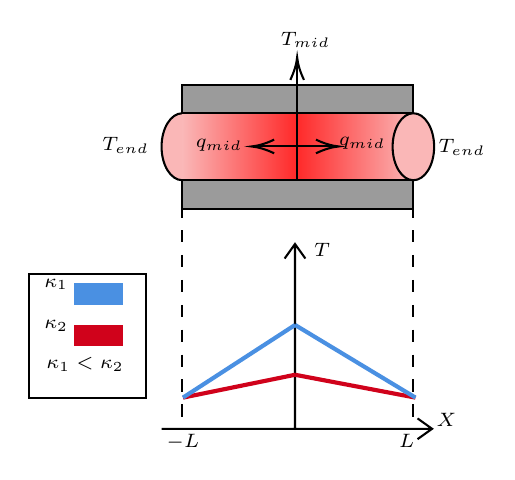
\begin{tikzpicture}[x=0.75pt,y=0.75pt,yscale=-1,xscale=1]
%uncomment if require: \path (0,300); %set diagram left start at 0, and has height of 300

%Shape: Ellipse [id:dp9620775434301283] 
\draw  [fill={rgb, 255:red, 250; green, 183; blue, 183 }  ,fill opacity=1 ] (90,75.87) .. controls (90,66.96) and (94.48,59.73) .. (100,59.73) .. controls (105.52,59.73) and (110,66.96) .. (110,75.87) .. controls (110,84.78) and (105.52,92) .. (100,92) .. controls (94.48,92) and (90,84.78) .. (90,75.87) -- cycle ;
%Shape: Rectangle [id:dp6239956030005828] 
\draw  [draw opacity=0][shading=_fyg9w4knt,_3b366t10c] (100,59.73) -- (211.33,59.73) -- (211.33,91.73) -- (100,91.73) -- cycle ;
%Shape: Rectangle [id:dp08450027404715932] 
\draw  [fill={rgb, 255:red, 155; green, 155; blue, 155 }  ,fill opacity=1 ] (100,46) -- (211.33,46) -- (211.33,59.73) -- (100,59.73) -- cycle ;
%Shape: Rectangle [id:dp030760279476271357] 
\draw  [fill={rgb, 255:red, 155; green, 155; blue, 155 }  ,fill opacity=1 ] (100,92) -- (211.33,92) -- (211.33,105.73) -- (100,105.73) -- cycle ;
%Shape: Ellipse [id:dp6410300181637909] 
\draw  [fill={rgb, 255:red, 250; green, 183; blue, 183 }  ,fill opacity=1 ] (201.33,75.87) .. controls (201.33,66.96) and (205.81,59.73) .. (211.33,59.73) .. controls (216.86,59.73) and (221.33,66.96) .. (221.33,75.87) .. controls (221.33,84.78) and (216.86,92) .. (211.33,92) .. controls (205.81,92) and (201.33,84.78) .. (201.33,75.87) -- cycle ;
%Straight Lines [id:da546691468990532] 
\draw    (155.33,34.73) -- (155.33,91.73) ;
\draw [shift={(155.33,32.73)}, rotate = 90] [color={rgb, 255:red, 0; green, 0; blue, 0 }  ][line width=0.75]    (10.93,-3.29) .. controls (6.95,-1.4) and (3.31,-0.3) .. (0,0) .. controls (3.31,0.3) and (6.95,1.4) .. (10.93,3.29)   ;
%Straight Lines [id:da4067263221168279] 
\draw    (155.67,75.73) -- (173.33,75.73) ;
\draw [shift={(175.33,75.73)}, rotate = 180] [color={rgb, 255:red, 0; green, 0; blue, 0 }  ][line width=0.75]    (10.93,-3.29) .. controls (6.95,-1.4) and (3.31,-0.3) .. (0,0) .. controls (3.31,0.3) and (6.95,1.4) .. (10.93,3.29)   ;
%Straight Lines [id:da5364570928647565] 
\draw    (155.67,75.73) -- (135.33,75.73) ;
\draw [shift={(133.33,75.73)}, rotate = 360] [color={rgb, 255:red, 0; green, 0; blue, 0 }  ][line width=0.75]    (10.93,-3.29) .. controls (6.95,-1.4) and (3.31,-0.3) .. (0,0) .. controls (3.31,0.3) and (6.95,1.4) .. (10.93,3.29)   ;
%Shape: Axis 2D [id:dp26845205848355935] 
\draw  (90,211.76) -- (220.33,211.76)(154.3,122.73) -- (154.3,212) (213.33,206.76) -- (220.33,211.76) -- (213.33,216.76) (149.3,129.73) -- (154.3,122.73) -- (159.3,129.73)  ;
%Straight Lines [id:da10525684167373806] 
\draw [color={rgb, 255:red, 208; green, 2; blue, 27 }  ,draw opacity=1 ][line width=1.5]    (154.33,185.73) -- (100.33,196.73) ;
%Straight Lines [id:da1508811281863801] 
\draw [color={rgb, 255:red, 208; green, 2; blue, 27 }  ,draw opacity=1 ][line width=1.5]    (212.33,196.73) -- (154.33,185.73) ;
%Straight Lines [id:da926366674445905] 
\draw [color={rgb, 255:red, 74; green, 144; blue, 226 }  ,draw opacity=1 ][line width=1.5]    (154.33,161.73) -- (100.33,196.73) ;
%Straight Lines [id:da48496756084972625] 
\draw [color={rgb, 255:red, 74; green, 144; blue, 226 }  ,draw opacity=1 ][line width=1.5]    (154.33,161.73) -- (212.33,196.73) ;
%Straight Lines [id:da9539282308371912] 
\draw  [dash pattern={on 4.5pt off 4.5pt}]  (211.33,92) -- (211.33,211.73) ;
%Straight Lines [id:da5241444385562701] 
\draw  [dash pattern={on 4.5pt off 4.5pt}]  (100,92) -- (100,211.73) ;
%Shape: Rectangle [id:dp7180380607123393] 
\draw  [draw opacity=0][fill={rgb, 255:red, 74; green, 144; blue, 226 }  ,fill opacity=1 ] (48,141.73) -- (71.33,141.73) -- (71.33,152) -- (48,152) -- cycle ;
%Shape: Rectangle [id:dp1387851277373967] 
\draw  [draw opacity=0][fill={rgb, 255:red, 208; green, 2; blue, 27 }  ,fill opacity=1 ] (48,161.73) -- (71.33,161.73) -- (71.33,172) -- (48,172) -- cycle ;
%Shape: Rectangle [id:dp6547879607723921] 
\draw   (26,137) -- (82.33,137) -- (82.33,196.73) -- (26,196.73) -- cycle ;

% Text Node
\draw (146,19) node [anchor=north west][inner sep=0.75pt]  [font=\scriptsize]  {$T_{mid}$};
% Text Node
\draw (222,71) node [anchor=north west][inner sep=0.75pt]  [font=\scriptsize]  {$T_{end}$};
% Text Node
\draw (60,70) node [anchor=north west][inner sep=0.75pt]  [font=\scriptsize]  {$T_{end}$};
% Text Node
\draw (105,70.73) node [anchor=north west][inner sep=0.75pt]  [font=\scriptsize]  {$q_{mid}$};
% Text Node
\draw (174,69.73) node [anchor=north west][inner sep=0.75pt]  [font=\scriptsize]  {$q_{mid}$};
% Text Node
\draw (162,121) node [anchor=north west][inner sep=0.75pt]  [font=\scriptsize]  {$T$};
% Text Node
\draw (221,203) node [anchor=north west][inner sep=0.75pt]  [font=\scriptsize]  {$X$};
% Text Node
\draw (203,213) node [anchor=north west][inner sep=0.75pt]  [font=\scriptsize]  {$L$};
% Text Node
\draw (91,213) node [anchor=north west][inner sep=0.75pt]  [font=\scriptsize]  {$-L$};
% Text Node
\draw (32,138) node [anchor=north west][inner sep=0.75pt]  [font=\scriptsize]  {$\kappa _{1}$};
% Text Node
\draw (32,158) node [anchor=north west][inner sep=0.75pt]  [font=\scriptsize]  {$\kappa _{2}$};
% Text Node
\draw (33,176) node [anchor=north west][inner sep=0.75pt]  [font=\scriptsize]  {$\kappa _{1} < \kappa _{2}$};
\end{tikzpicture}
\caption{A metal rod with fixed end temperature(top), and its steady-state temperature profiles along axial direction(bottom) when it's made of two distinct materials with thermal conductivity coefficient being $\kappa_1$ and $\kappa_2$, respectively.}
\label{fig4-1}
\end{marginfigure}
At the steady state, we ignore temperature variation at radial direction, and obtain a mountain-like temperature profile along the axial direction (see the bottom profiles in Fig.\ref{fig4-1}). With the constant $q_{mid}$, the "steepness" of temperature profile decreases as the thermal conductivity coefficient $\kappa$ increases according to Fourier's law. As a result, the "height" of our mountain will decrease if the rod is made of materials that have larger thermal conductivity coefficient. We thus conclude that to make temperature variation inside heated body negligible, \textbf{the body needs to be highly thermal-conductive.}

\subsection{Biot number}
\imp{Being small and thermal-conductive is \textbf{NOT ENOUGH} for a heated body to be treated as lumped resistance or capacitance}, because so far, we deliberately overlooked the effects of convection at the two ends of the rod in the thought experiment above. Now, if we allow $T_{end}$ to vary by exposing the two ends to an ambient environment. If the ambient temperature $T_{\infty}$ is fixed, then the convective flux at the two ends are $q_{conv}=h(T_{end}-T_{\infty})$, where $h$ is convective heat transfer coefficient. Let $L$ be the distance from the middle point to the rod end. Then, at the steady state, we establish conservation of energy in left(and right) half of the rod as

\begin{equation}
\begin{aligned}
    q_{mid}&=q_{conv}\\
    \kappa\frac{T_{mid}-T_{end}}{L}&=h(T_{end}-T_{\infty})
\end{aligned}
\label{eqn4-1}
\end{equation}
where $T_{mid}$ is the middle-point temperature, and Fourier's Law and Newton's cooling law are used at the second equivalence. If all the temperatures in Eq.(\ref{eqn4-1}) are moved to LHS, we get a dimensionless number at RHS, which is named after the French physicist \textbf{Jean-Baptiste Biot}\footnote{\href{https://en.wikipedia.org/wiki/Jean-Baptiste_Biot}{Biot on Wikipedia}}\index{Biot number}, i.e.,

\begin{equation}
    \frac{T_{mid}-T_{end}}{T_{end}-T_{\infty}}=\frac{hL}{\kappa}.
    \label{eq4-2}
\end{equation}
With the relation in Eq.(\ref{eq4-2}), we are now ready to use \textbf{Biot number} to judge whether a heated body can be treated as a lumped component. Because we require lumped components to have only negligible internal temperature gradient, $T_{mid}-T_{end}$ must be small (i.e. $T_{mid}-T_{end}\approx0$). Since $T_{end}>T_{\infty}$ when the body is heated up, \textbf{the smaller the Biot number is, the more accurate the assumption of lumped component becomes.} A rule of thumb is that we can treat a body as a lumped capacitance/resistance, if its Biot number $Bi=\frac{hL}{\kappa}<0.1$.

\subsection{Nussalt number and thermal conductivity of fluid}
It is not uncommon that people mistake Nussalt number with Biot number, because they have identical expression at first sight. While Biot number can be heuristically understood as a ratio of $\frac{\text{surface convection}}{\text{conduction in solid}}$, Nussalt number\index{Nussalt number} describes heat transfer solely inside the fluid body. Therefore, the thermal conductivity coefficient in Eq.(\ref{eq4-3}) is a property of the fluid in contact with a solid surface.
\begin{equation}
    Nu=\frac{hL}{k_{fluid}}.
    \label{eq4-3}
\end{equation}
A simple derivation of Nussalt number is given as following: Let us imagine a heated solid surface is in contact with a fluid of thickness $L$. When the fluid flows steadily along the surface, the heat flux is then 

\begin{equation}
    q_{conv,fluid}=h(T_s-T_{fluid}),
\end{equation}
where $T_s$ and $T_{fluid}$ are the surface temperature and the temperature of fluid body. If there is no flow, on the other hand, the heat transfers to the fluid through heat conduction only to give
\begin{equation}
    q_{cond,fluid}=k_{fluid}\frac{T_{s}-T_{fluid}}{L}.
\end{equation}
The Nussalt number is then defined as the ratio of $\frac{\text{convection flux}}{\text{conduction flux}}$,i.e.,
\begin{equation}
    Nu=\frac{h(T_s-T_{fluid})}{k_{fluid}\frac{(T_{s}-T_{fluid})}{L}}=\frac{hL}{k_{fluid}}.
\end{equation}

For readers who enjoyed the discussion in Lab2, there is something off regarding the conduction in the fluid. In lab2 we have discussed how the heat flux represented by the flow of electrons is not well-defined at the \textbf{interface between the solid and the ambient environment}, and thus, $q_{conv}=0$ is retained. Within the body of fluid, the conductive flux is, however, well-defined. Instead of having electron flow that carries thermal energy in solid, \imp{the heat conduction in fluid is accomplished by the energy exchange between adjacent molecules.} For a polyatomic molecules\footnote{In fact, it is possible to derive thermal conductivity coefficient from statistically averaged molecular properties, such as mean free path and mean molecular velocities. The methods used for such derivation is under the study of a subject called "statistical mechanics"}, the energy exchange (or collisions) causes changes in vibrational and rotational frequencies, and translational velocities. The table below lists thermal conductivity of some common gases.

\begin{table}[h]
\begin{center}
\tiny
\begin{tabular}{llllllll}
                            &                             & \multicolumn{6}{l}{Thermal conductivity coefficient in $mWm^{-1}K^{-1}$} \\ \hline
\multicolumn{1}{l|}{}       &                             & 100 K      & 200 K      & 300 K      & 400 K     & 500 K     & 600 K     \\ \hline
\multicolumn{1}{l|}{}       & Air                         & 9.5        & 18.5       & 26.4       & 33.5      & 39.9      & 46.0      \\
\multicolumn{1}{l|}{$Ar$}   & Argon (P = 0)               & 6.3        & 12.4       & 17.7       & 22.4      & 26.5      & 30.3      \\
\multicolumn{1}{l|}{$BF_3$} & Boron trifluoride           &            &            & 19.0       & 24.6      &           &           \\
\multicolumn{1}{l|}{$HCl$}  & Hydrogen chloride           &            & 9.2        & 14.5       & 19.5      & 24.0      & 28.1      \\
\multicolumn{1}{l|}{$F_6S$} & Sulfur hexafluoride (P = 0) &            &            & 13.0       & 20.6      & 27.5      & 33.8      \\
\multicolumn{1}{l|}{$H_2$}  & Normal hydrogen (P = 0)     & 68.2       & 132.8      & 186.6      & 230.9     & 270.9     & 309.1     \\
\multicolumn{1}{l|}{$H_2O$} & Water (P=0)                 &            &            & 18.6       & 26.1      & 35.6      & 46.2      \\
\multicolumn{1}{l|}{$D_2O$} & Deuterium oxide (P = 0)     &            &            & 18.2       & 26.6      & 36.3      & 47.6      \\
\multicolumn{1}{l|}{$H_2S$} & Hydrogen sulfide            &            &            & 14.6       & 20.5      & 26.4      & 32.4      \\
\multicolumn{1}{l|}{$H_3N$} & Ammonia                     &            &            & 25.1       & 37.2      & 53.1      & 68.6      \\
\multicolumn{1}{l|}{$He$}   & Helium (P = 0)              & 74.7       & 118.3      & 155.7      & 189.6     & 221.4     & 251.6     \\
\multicolumn{1}{l|}{$Kr$}   & Krypton (P = 0)             &            & 6.5        & 9.5        & 12.3      & 14.8      & 17.1      \\
\multicolumn{1}{l|}{$NO$}   & Nitric oxide                &            & 17.8       & 25.9       & 33.1      & 39.6      & 46.2      \\
\multicolumn{1}{l|}{$N_2$}  & Nitrogen                    & 9.4        & 18.3       & 26.0       & 32.8      & 39.0      & 44.8      \\
\multicolumn{1}{l|}{$N_2O$} & Nitrous oxide               &            & 9.8        & 17.4       & 26.0      & 34.1      & 41.8\\
\hline
\end{tabular}
\caption{\href{https://www.nist.gov/publications/thermal-conductivity-gases}{Tabulated data of thermal conductivity from NIST.} Unless otherwise stated, the measurements are taken under 1 standard atmosphere pressure. The notation "P=0" indicates that the low-pressure limiting value is given.}
\label{tab4-1}
\end{center}
\end{table}

From Table \ref{tab4-1}, we see that the thermal conductivity coefficient of gases increases with temperature. To explain such phenomenon, \imp{it is not sufficient, however, to resort to ideal gas law}\index{ideal gas law},
\begin{equation}
    PV=nRT.
    \label{eq4-7}
\end{equation}
Because most of the data in Table \ref{tab4-1} are obtained with the pressure $P$ fixed at 1 bar, an increase in ambient temperature results in volumetric expansion, reducing the gas number density $\rho=n/V$.\index{number density} Since reduced $\rho$ indicates that gaseous molecule need to travel longer distance before its next collision, the ideal gas law seems to tell us that the rate of molecular energy exchange is quenched at high temperature, resulting decreasing thermal conductivity coefficient.

A heuristic correction to this contradictory explanation lies in the increased kinetic energy of gaseous molecules at high temperature. The excess of kinetic energy promotes the rate of collision despite of the increased distance between molecules, and hence, the rate of energy exchanges is also increased. For readers interested in a more quantitative relationship between temperature and thermal conductivity, a short account of the kinetic theory of monoatomic gas is prepared at the end of current chapter.

\section{Cooling and heating lumped components}
Now that we are persuaded that heated bodied with $Bi<0.1$ are lumped component, it is easy to write down a governing equation, and the solution to it tells transient temperature variation of lumped body over time. Notice that the assumption of lumped component gives us the freedom of ignoring heat conduction inside heated body. So we can establish a conservation of energy by only considering the convection at solid surface, i.e., the thermal energy change in lumped component $\Delta Q$ is solely caused by the convective heat flux $q_{conv}$ on the solid surface of area "$A$". From Eq.(\ref{eq2-3}), we have
\begin{equation}
    \Delta Q=mc_p(T_{init}-T_{body})=q_{conv}Adt,
    \label{eq4-8}
\end{equation}
where $T_{init}$ and $T_{body}$ are initial and current temperature in the lumped component body of interest\footnote{Remember that $c_p$ is specific heat}. Using Newton's cooling law at RHS of Eq.(\ref{eq4-8}) gives
\begin{equation}
    \frac{mc_p(T_{init}-T_{body})}{dt}=hA(T_{body}-T_{\infty})
    \label{eq4-9},
\end{equation}
where the surface temperature is replaced with $T_{body}$ at RHS due to the assumption of lumped body. Now we divide both sides of (\ref{eq4-9}) by $T_{init}-T_{\infty}$ and write LHS as a first-order derivation with respect to time, which results in
\begin{equation}
    -\frac{mc_p}{(T_{init}-T_{\infty})}\frac{dT_{body}}{dt}=hA\frac{T_{body}-T_{\infty}}{T_{init}-T_{\infty}}
    \label{eq4-10}.
\end{equation}
Since $(T_{init}-T_{\infty})$ is a constant, Eq.(\ref{eq4-10}) can be written as an ordinary differential equation (ODE) of the normalized temperature\index{normalized temperature}, $\theta=\frac{T_{body}-T_{\infty}}{T_{init}-T_{\infty}}$, as
\begin{equation}
    -mc_p\frac{d\theta}{dt}=hA\theta
    \label{eq4-11}.
\end{equation}
Eq.(\ref{eq4-11}) has a simple solution of exponential function,i.e.,
\begin{equation}
    \theta=exp\left(-\frac{hA}{mc_p}t\right)=exp(-\alpha t).
    \label{eq4-12}
\end{equation}
Here the constant $\alpha$ (its inverse $\tau=1/\alpha$ is sometimes referred as time constant\index{time constant}) can be further simplified by writing the volume of lumped body, $V$, as a product of its surface area $A$ exposed to fluid, and the inverse of its \imp{\textbf{surface-to-volume ratio}}\index{surface-to-volume ratio} $r_{sv}$ (i.e., $V=A/r_{sv}$). So Eq.(\ref{eq4-12}) becomes
\begin{equation}
    \theta=exp\left(-\frac{hr_{sv}}{\rho_sc_p}t\right)
    \label{eq4-13}
\end{equation}
with $\rho_s$ being the density of lumped component of interest. Eq.(\ref{eq4-13}) sometimes is referred as power-law function\index{power-law function} of lumped component. It clearly shows that the transient temperature variation of lumped components \imp{has nothing to do with the thermal conductivity coefficient.} Instead, the variation is controlled by (1) convective transfer coefficient,(2) surface-to-volume ratio, (3) solid density, and (4) specific heat. \imp{Any action that reduces inverse time constant "$\alpha$" will slow down the cooling process of lumped component.} Fig.\ref{fig4-2} shows that the reduction in $T_{body}$ within first 4 units of time is the most significant when the constant $\alpha$ is the largest.
\begin{marginfigure}
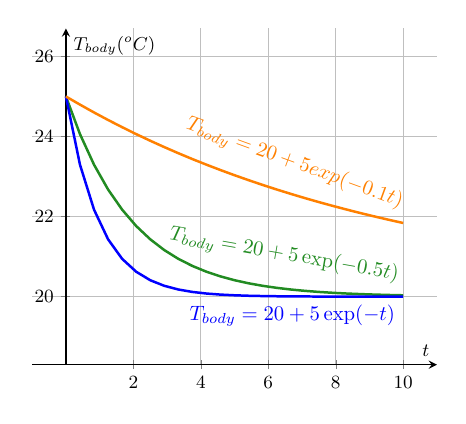
\begin{tikzpicture}[x=0.75pt,y=0.75pt,yscale=0.75,xscale=0.75]
\begin{axis}[grid=both,
          xmax=10,ymax=26,ymin=19,
          axis lines=middle,
          restrict y to domain=0:26,
          restrict x to domain=0:10,
          every axis plot/.append style={very thick},
          xlabel=$t$,
          ylabel=$T_{body}({}^oC)$,
          label style={font=\small},
          tick label style={font=\small},
          enlargelimits]
\addplot[ForestGreen,domain=0:10]  {20+5*exp(-0.5*x)} node[above left,rotate=-10]{$T_{body}=20+5\exp(-0.5t)$};
\addplot[blue,domain=0:10]  {20+5*exp(-x)} node[below left] {$T_{body}=20+5\exp(-t)$};
\addplot[orange,domain=0:10]{20+5*exp(-0.1*x)} node[above left,rotate=-20] {$T_{body}=20+5exp(-0.1t)$};
\end{axis}
\end{tikzpicture}
\caption{Temperature profiles as a function of time "$t$" with $T_{\infty}=20{}^oC$, $T_{init}-T_{\infty}=5{}^oC$, and time constant $\alpha=1$(blue),$0.5$(green), and $0.1$(orange).}
\label{fig4-2}
\end{marginfigure}
The discussion above can be readily applied to the heating process of lumped component. To see this, we write out temperatures explicitly in Eq.(\ref{eq4-13}) as
\begin{equation}
    T_{body}=T_{\infty}+\left(T_{init}-T_{\infty}\right)exp\left(-\frac{hr_{sv}}{\rho_sc_p}t\right).
    \label{eq4-14}
\end{equation}
When the ambient temperature $T_{\infty}$ is higher than the lumped body temperature $T_{body}$, Eq. (\ref{eq4-14}) describes temperature variation of a heating process, and a cooling process otherwise. Fig.\ref{fig4-3} shows that the temperature profiles of a cooling and a heating process are mirror images to each other when $|T_{int}-T_{\infty}|=3^oC$.
\begin{marginfigure}
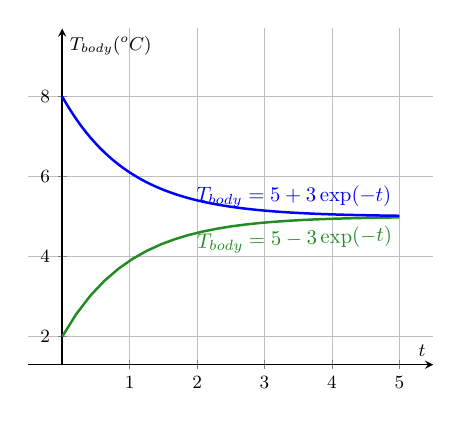
\begin{tikzpicture}[x=0.75pt,y=0.75pt,yscale=0.75,xscale=0.75]
\begin{axis}[grid=both,
          xmax=5,ymax=9,
          axis lines=middle,
          restrict y to domain=0:10,
          restrict x to domain=0:7,
          every axis plot/.append style={very thick},
          xlabel=$t$,
          ylabel=$T_{body}({}^oC)$,
          label style={font=\small},
          tick label style={font=\small},
          enlargelimits]
\addplot[ForestGreen,domain=0:5]  {5-3*exp(-x)} node[below left,rotate=2]{$T_{body}=5-3\exp(-t)$};
\addplot[blue,domain=0:5,samples=100]  {5+3*exp(-x)} node[above left] {$T_{body}=5+3\exp(-t)$};
\end{axis}
\end{tikzpicture}
\caption{Cooling(bottom) and heating(top) process with $|T_{init}-T_{\infty}|=3^oC$ and $T_{\infty}=5^oC$}
\label{fig4-3}
\end{marginfigure}
\subsection{Effects of material properties on convection}
Things become more interesting if we pay extra attention to the four factors in inverse time constant $\alpha$\index{inverse time constant}, and their effects on the cooling/heating rate of lumped component. From Eq. (\ref{eq4-13}), the density $\rho_s$ and the specific heat $c_p$ are two intrinsic material properties, and product of the two varies with material types. The table below lists the values of $\rho_sc_p$ for some common matallic and ceramic materials.
\begin{table}[h]
\small
\begin{tabular}{c|ccc}
\hline
Material & Specific heat(kJ/kgK) & Density(kg/m3) & $c_p\rho_s$ \\ \hline
Aluminum & 0.9                   & 2550           & 2295        \\
Brass    & 0.375                 & 8730           & 3273.75     \\
Stainless steel    & 0.49                  & 8030           & 3934.7      \\
Macor    & 0.79                  & 2520           & 1990.8      \\ \hline
\end{tabular}
\caption{Specific heat and density of some common materials, the data for machinable glass ceramic "Macor" is obtained from \href{https://www.corning.com/worldwide/en/products/advanced-optics/product-materials/specialty-glass-and-glass-ceramics/glass-ceramics/macor.html}{Corning Inc.}}
\label{tab4-2}
\end{table}
If we fix the values of $h$ and $r_{sv}$, Table \ref{tab4-2} shows that steel and Macor have the smallest and the largest inverse time constant $\alpha$, respectively. Starting from the same initial temperature, the rank of cooling/heating rates for these materials follows a sequence of Macor\index{Macor}>Aluminum>Brass>Stainless steel.
\subsection{Effects of geometry of lumped components on convection}
There is no way to fit a decent discussion of the relationship between convective coefficient $h$ with other physical parameters in this note\footnote{Up to March 24th, 2021, there are in total 1,360,000 research papers related to "convective coefficient" available on Google scholar}, which left us with the last factor in $\alpha$: the surface-to-volume ratio, $r_{sv}$. For some highly symmetric shapes, such as sphere and cube, if we assume that the whole lumped body is exposed to convective process, then $r_{sv}$ can be readily calculated by using formula listed in Table \ref{tab4-3}.
\begin{table}[h]
\begin{center}
\small
\begin{tabular}{c|cc}
\hline
Geometry     & Vol.             & $r_{sv}$       \\ \hline
Tetrahedron  & $\sqrt{2}a^3/12$ & ${14.697}/{a}$ \\
Octahedron   & $\sqrt{2}a^3/3$  & ${7.348}/{a}$  \\
Cube         &      $a^3$       & ${6}/{a}$      \\
Sphere       &   $4\pi a^3/3$   & ${3}/{a}$      \\
Dodecahedron &$(15+7\sqrt{5})a^{3}/4$& ${2.694}/{a}$  \\ \hline
\end{tabular}
\end{center}
\caption{$r_{sv}$ of common shapes with $a$ being the length of edge/radius}\
\label{tab4-3}
\end{table}
With these formula, we can also plot $r_{sv}$ against the volumes of these shapes in Fig.\ref{fig4-4}. This simple analysis shows that for a given volume of lumped component, tetrahedron has the largest $r_{sv}$ while sphere has the smallest. Because large $r_{sv}$ results in large $\alpha$, Fig.\ref{fig4-2} and \ref{fig4-4} indicate that \imp{the $T_{body}$ drops(cooling) and increases(heating) much quicker in a tetrahedral body than in a spherical body}. As the lumped body becomes more and more bulky, $r_{sv}$ of all kinds of polyhedral bodies decrease in an order of $O(1/x)$, resulting in more sluggish cooling and heating process. Of course, the bulky component also undermines the validity of lumped capacitance assumption.

\begin{marginfigure}[0in]
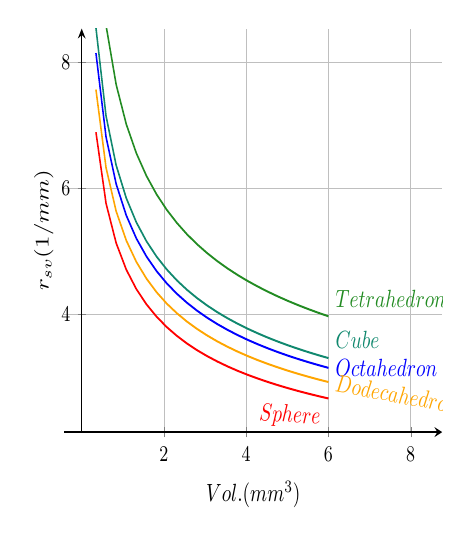
\begin{tikzpicture}[x=0.7pt,y=0.9pt,yscale=0.9,xscale=0.70]
\begin{axis}[grid=both,
          xmax=8,ymax=8,
          axis lines=middle,
          restrict y to domain=0:9,
          restrict x to domain=0:7,
          every axis plot/.append style={ thick},
          xlabel=$Vol.(mm^3)$,
          x label style={at={(axis description cs:0.5,-0.1)},anchor=north},
          y label style={at={(axis description cs:-0.01,.5)},rotate=90,anchor=south},
          ylabel=$r_{sv}(1/mm)$,
          label style={font=\normalsize},
          tick label style={font=\small},
          enlargelimits]
\addplot[ForestGreen,domain=0.1:6]  {14.697/(12*x/sqrt(2))^0.3333} node[above right]{$Tetrahedron$};
\addplot[Blue,domain=0.1:6]  {7.348/(3*x/sqrt(2))^0.3333} node[ right]{$Octahedron$};
\addplot[PineGreen,domain=0.1:6]  {6/(x)^0.3333} node[above right]{$Cube$};
\addplot[red,domain=0.1:6]  {3/(3*x/(4*3.1415926))^0.3333} node[below left,rotate=-3]{$Sphere$};
\addplot[Orange,domain=0.1:6]  {2.694/(4*x/(15+7*sqrt(5)))^0.3333} node[ right,rotate=-8]{$Dodecahedron$};
\end{axis}
\end{tikzpicture}
\caption{$r_{sv}$ versus polyhedral volumes}
\label{fig4-4}
\end{marginfigure}

\section{A kinetic theory for thermal conductivity of gas}
\begin{docspec}
TL;DR: I indulged myself to write this section only because deriving macroscopic law from statistical behavior of molecules is intellectually satisfying. For impatient readers, please check the most important results at the end. For ambitious readers, please refer to Sears' book for accessible introduction to statistical thermodynamics\cite{sears1975thermodynamics}, and C.V. Heer's account of stochastic perspectives of thermal physics\cite{heer2012statistical}.
\end{docspec}

To simplify our derivation without losing generality, we again employ some of the assumptions introduced in Lab1, and they are
\renewcommand{\labelenumi}{\Roman{enumi}.}
\begin{enumerate}
	\item gas molecules are treated as hard spherical mass of radius $ r $, and
	\item potential energy of each molecule is negligible.
\end{enumerate}
Careful readers might find that assumption \rom{1} is now considering molecular volumes comparing to the old one.  In lab1, we only care about the collision between molecules and the wall of container where the cross section of single molecule is negligible. Inside the body of a container, where molecules collide with each other, making molecular size finite helps to visualize process of momentum/energy exchange and to calculate important physical quantities that describe molecular motions. One of such physical quantities is the so-called \imp{mean free path}(MFP)\index{mean free path}, which measures on average the distance a gas molecule needs to travel before it collides with another molecule. Knowing MFP is important for our purpose of relating thermal conductivity to molecular motions.As we will show in later sections, viscosity and conductivity stem from momentum and energy exchange between adjacent gas molecules, and MFT provides a measurement of how often such exchanges could happen and bridges thermal conductivity with other thermodynamic quantities (i.e. state parameters).  So let's start by deriving a simple expression for MFP below.

\subsection{Scattering and Mean free path }
From the assumption \rom{1}, we can define the exclusion volume for single molecule as $ 4\pi r^3/3 $, i.e., two gas molecules can not have overlap in their molecular volumes. Let us now consider a thin slice of thickness $ \Delta x $ in a cubic container of edge length $ L $. The slice is thin enough so that molecules contained in the slice does not overlap with each other long $ x- $dimension (see Fig. \ref{fig:target-bullet}).
\begin{marginfigure}
	\tikzset{every picture/.style={line width=0.75pt}} %set default line width to 0.75pt        
	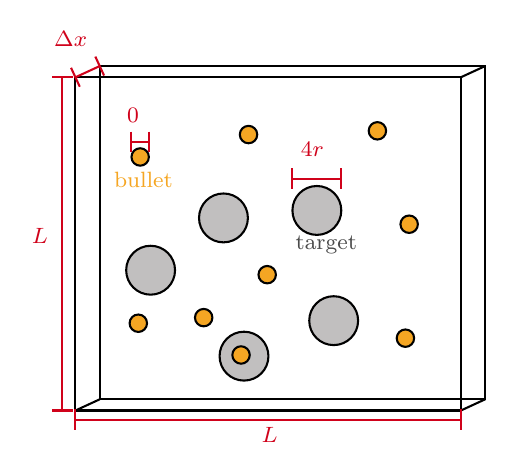
\begin{tikzpicture}[x=0.75pt,y=0.75pt,yscale=-0.9,xscale=0.9]
		%uncomment if require: \path (0,300); %set diagram left start at 0, and has height of 300
		
		%Shape: Rectangle [id:dp14429340171670446] 
		\draw   (359,51) -- (565.33,51) -- (565.33,229.4) -- (359,229.4) -- cycle ;
		%Shape: Rectangle [id:dp32354541052017527] 
		\draw   (372,45) -- (578.33,45) -- (578.33,223.4) -- (372,223.4) -- cycle ;
		%Straight Lines [id:da7074428847272893] 
		\draw [color={rgb, 255:red, 208; green, 2; blue, 27 }  ,draw opacity=1 ]   (359,51) -- (372,45) ;
		\draw [shift={(372,45)}, rotate = 515.22] [color={rgb, 255:red, 208; green, 2; blue, 27 }  ,draw opacity=1 ][line width=0.75]    (0,5.59) -- (0,-5.59)   ;
		\draw [shift={(359,51)}, rotate = 515.22] [color={rgb, 255:red, 208; green, 2; blue, 27 }  ,draw opacity=1 ][line width=0.75]    (0,5.59) -- (0,-5.59)   ;
		%Straight Lines [id:da9764043397060111] 
		\draw    (359,229.4) -- (372,223.4) ;
		%Straight Lines [id:da7488556721129279] 
		\draw    (565.33,229.4) -- (578.33,223.4) ;
		%Straight Lines [id:da5942213972622079] 
		\draw    (565.33,51) -- (578.33,45) ;
		%Shape: Circle [id:dp13513954211829737] 
		\draw  [fill={rgb, 255:red, 193; green, 191; blue, 191 }  ,fill opacity=1 ] (475.17,122.28) .. controls (475.17,115.06) and (481.02,109.2) .. (488.25,109.2) .. controls (495.48,109.2) and (501.33,115.06) .. (501.33,122.28) .. controls (501.33,129.51) and (495.48,135.37) .. (488.25,135.37) .. controls (481.02,135.37) and (475.17,129.51) .. (475.17,122.28) -- cycle ;
		%Straight Lines [id:da6896831294830664] 
		\draw [color={rgb, 255:red, 208; green, 2; blue, 27 }  ,draw opacity=1 ]   (475.17,105.28) -- (501.33,105.28) ;
		\draw [shift={(501.33,105.28)}, rotate = 180] [color={rgb, 255:red, 208; green, 2; blue, 27 }  ,draw opacity=1 ][line width=0.75]    (0,5.59) -- (0,-5.59)   ;
		\draw [shift={(475.17,105.28)}, rotate = 180] [color={rgb, 255:red, 208; green, 2; blue, 27 }  ,draw opacity=1 ][line width=0.75]    (0,5.59) -- (0,-5.59)   ;
		%Shape: Circle [id:dp6999071649743681] 
		\draw  [fill={rgb, 255:red, 193; green, 191; blue, 191 }  ,fill opacity=1 ] (425.17,126.28) .. controls (425.17,119.06) and (431.02,113.2) .. (438.25,113.2) .. controls (445.48,113.2) and (451.33,119.06) .. (451.33,126.28) .. controls (451.33,133.51) and (445.48,139.37) .. (438.25,139.37) .. controls (431.02,139.37) and (425.17,133.51) .. (425.17,126.28) -- cycle ;
		%Shape: Circle [id:dp8447371235394252] 
		\draw  [fill={rgb, 255:red, 193; green, 191; blue, 191 }  ,fill opacity=1 ] (484.17,181.28) .. controls (484.17,174.06) and (490.02,168.2) .. (497.25,168.2) .. controls (504.48,168.2) and (510.33,174.06) .. (510.33,181.28) .. controls (510.33,188.51) and (504.48,194.37) .. (497.25,194.37) .. controls (490.02,194.37) and (484.17,188.51) .. (484.17,181.28) -- cycle ;
		%Shape: Circle [id:dp9021087063137504] 
		\draw  [fill={rgb, 255:red, 245; green, 166; blue, 35 }  ,fill opacity=1 ] (423,179.67) .. controls (423,177.09) and (425.09,175) .. (427.67,175) .. controls (430.24,175) and (432.33,177.09) .. (432.33,179.67) .. controls (432.33,182.24) and (430.24,184.33) .. (427.67,184.33) .. controls (425.09,184.33) and (423,182.24) .. (423,179.67) -- cycle ;
		%Shape: Circle [id:dp26186478190204787] 
		\draw  [fill={rgb, 255:red, 245; green, 166; blue, 35 }  ,fill opacity=1 ] (533,129.67) .. controls (533,127.09) and (535.09,125) .. (537.67,125) .. controls (540.24,125) and (542.33,127.09) .. (542.33,129.67) .. controls (542.33,132.24) and (540.24,134.33) .. (537.67,134.33) .. controls (535.09,134.33) and (533,132.24) .. (533,129.67) -- cycle ;
		%Shape: Circle [id:dp5362736059677999] 
		\draw  [fill={rgb, 255:red, 245; green, 166; blue, 35 }  ,fill opacity=1 ] (389,93.67) .. controls (389,91.09) and (391.09,89) .. (393.67,89) .. controls (396.24,89) and (398.33,91.09) .. (398.33,93.67) .. controls (398.33,96.24) and (396.24,98.33) .. (393.67,98.33) .. controls (391.09,98.33) and (389,96.24) .. (389,93.67) -- cycle ;
		%Shape: Circle [id:dp22591518852148873] 
		\draw  [fill={rgb, 255:red, 245; green, 166; blue, 35 }  ,fill opacity=1 ] (516,79.67) .. controls (516,77.09) and (518.09,75) .. (520.67,75) .. controls (523.24,75) and (525.33,77.09) .. (525.33,79.67) .. controls (525.33,82.24) and (523.24,84.33) .. (520.67,84.33) .. controls (518.09,84.33) and (516,82.24) .. (516,79.67) -- cycle ;
		%Shape: Circle [id:dp5354524164848686] 
		\draw  [fill={rgb, 255:red, 245; green, 166; blue, 35 }  ,fill opacity=1 ] (457,156.67) .. controls (457,154.09) and (459.09,152) .. (461.67,152) .. controls (464.24,152) and (466.33,154.09) .. (466.33,156.67) .. controls (466.33,159.24) and (464.24,161.33) .. (461.67,161.33) .. controls (459.09,161.33) and (457,159.24) .. (457,156.67) -- cycle ;
		%Shape: Circle [id:dp8445769418144385] 
		\draw  [fill={rgb, 255:red, 245; green, 166; blue, 35 }  ,fill opacity=1 ] (447,81.67) .. controls (447,79.09) and (449.09,77) .. (451.67,77) .. controls (454.24,77) and (456.33,79.09) .. (456.33,81.67) .. controls (456.33,84.24) and (454.24,86.33) .. (451.67,86.33) .. controls (449.09,86.33) and (447,84.24) .. (447,81.67) -- cycle ;
		%Shape: Circle [id:dp5082335629816249] 
		\draw  [fill={rgb, 255:red, 245; green, 166; blue, 35 }  ,fill opacity=1 ] (531,190.67) .. controls (531,188.09) and (533.09,186) .. (535.67,186) .. controls (538.24,186) and (540.33,188.09) .. (540.33,190.67) .. controls (540.33,193.24) and (538.24,195.33) .. (535.67,195.33) .. controls (533.09,195.33) and (531,193.24) .. (531,190.67) -- cycle ;
		%Shape: Circle [id:dp9902014886485704] 
		\draw  [fill={rgb, 255:red, 245; green, 166; blue, 35 }  ,fill opacity=1 ] (388,182.67) .. controls (388,180.09) and (390.09,178) .. (392.67,178) .. controls (395.24,178) and (397.33,180.09) .. (397.33,182.67) .. controls (397.33,185.24) and (395.24,187.33) .. (392.67,187.33) .. controls (390.09,187.33) and (388,185.24) .. (388,182.67) -- cycle ;
		%Shape: Circle [id:dp952119316749187] 
		\draw  [fill={rgb, 255:red, 193; green, 191; blue, 191 }  ,fill opacity=1 ] (436.17,200.28) .. controls (436.17,193.06) and (442.02,187.2) .. (449.25,187.2) .. controls (456.48,187.2) and (462.33,193.06) .. (462.33,200.28) .. controls (462.33,207.51) and (456.48,213.37) .. (449.25,213.37) .. controls (442.02,213.37) and (436.17,207.51) .. (436.17,200.28) -- cycle ;
		%Shape: Circle [id:dp9768621182270503] 
		\draw  [fill={rgb, 255:red, 193; green, 191; blue, 191 }  ,fill opacity=1 ] (386.17,154.28) .. controls (386.17,147.06) and (392.02,141.2) .. (399.25,141.2) .. controls (406.48,141.2) and (412.33,147.06) .. (412.33,154.28) .. controls (412.33,161.51) and (406.48,167.37) .. (399.25,167.37) .. controls (392.02,167.37) and (386.17,161.51) .. (386.17,154.28) -- cycle ;
		%Shape: Circle [id:dp5933956722813136] 
		\draw  [fill={rgb, 255:red, 245; green, 166; blue, 35 }  ,fill opacity=1 ] (443,199.67) .. controls (443,197.09) and (445.09,195) .. (447.67,195) .. controls (450.24,195) and (452.33,197.09) .. (452.33,199.67) .. controls (452.33,202.24) and (450.24,204.33) .. (447.67,204.33) .. controls (445.09,204.33) and (443,202.24) .. (443,199.67) -- cycle ;
		%Straight Lines [id:da39624072741998007] 
		\draw [color={rgb, 255:red, 208; green, 2; blue, 27 }  ,draw opacity=1 ]   (359,234.4) -- (565.33,234.4) ;
		\draw [shift={(565.33,234.4)}, rotate = 180] [color={rgb, 255:red, 208; green, 2; blue, 27 }  ,draw opacity=1 ][line width=0.75]    (0,5.59) -- (0,-5.59)   ;
		\draw [shift={(359,234.4)}, rotate = 180] [color={rgb, 255:red, 208; green, 2; blue, 27 }  ,draw opacity=1 ][line width=0.75]    (0,5.59) -- (0,-5.59)   ;
		%Straight Lines [id:da3003697992677039] 
		\draw [color={rgb, 255:red, 208; green, 2; blue, 27 }  ,draw opacity=1 ]   (352,51) -- (352,229.4) ;
		\draw [shift={(352,229.4)}, rotate = 270] [color={rgb, 255:red, 208; green, 2; blue, 27 }  ,draw opacity=1 ][line width=0.75]    (0,5.59) -- (0,-5.59)   ;
		\draw [shift={(352,51)}, rotate = 270] [color={rgb, 255:red, 208; green, 2; blue, 27 }  ,draw opacity=1 ][line width=0.75]    (0,5.59) -- (0,-5.59)   ;
		%Straight Lines [id:da9062896342290824] 
		\draw [color={rgb, 255:red, 208; green, 2; blue, 27 }  ,draw opacity=1 ]   (389,85.67) -- (398.33,85.67) ;
		\draw [shift={(398.33,85.67)}, rotate = 180] [color={rgb, 255:red, 208; green, 2; blue, 27 }  ,draw opacity=1 ][line width=0.75]    (0,5.59) -- (0,-5.59)   ;
		\draw [shift={(389,85.67)}, rotate = 180] [color={rgb, 255:red, 208; green, 2; blue, 27 }  ,draw opacity=1 ][line width=0.75]    (0,5.59) -- (0,-5.59)   ;
		
		% Text Node
		\draw (478,84) node [anchor=north west][inner sep=0.75pt]  [font=\footnotesize,color={rgb, 255:red, 208; green, 2; blue, 27 }  ,opacity=1 ]  {$4r$};
		% Text Node
		\draw (346,25) node [anchor=north west][inner sep=0.75pt]  [font=\footnotesize,color={rgb, 255:red, 208; green, 2; blue, 27 }  ,opacity=1 ]  {$\Delta x$};
		% Text Node
		\draw (457,237) node [anchor=north west][inner sep=0.75pt]  [font=\footnotesize,color={rgb, 255:red, 208; green, 2; blue, 27 }  ,opacity=1 ]  {$L$};
		% Text Node
		\draw (334,130) node [anchor=north west][inner sep=0.75pt]  [font=\footnotesize,color={rgb, 255:red, 208; green, 2; blue, 27 }  ,opacity=1 ]  {$L$};
		% Text Node
		\draw (385,66) node [anchor=north west][inner sep=0.75pt]  [font=\footnotesize,color={rgb, 255:red, 208; green, 2; blue, 27 }  ,opacity=1 ]  {$0$};
		% Text Node
		\draw (475.17,134.2) node [anchor=north west][inner sep=0.75pt]  [font=\footnotesize,color={rgb, 255:red, 74; green, 74; blue, 74 }  ,opacity=1 ] [align=left] {target};
		% Text Node
		\draw (378,100) node [anchor=north west][inner sep=0.75pt]  [font=\footnotesize,color={rgb, 255:red, 245; green, 166; blue, 35 }  ,opacity=1 ] [align=left] {bullet};
		
		
	\end{tikzpicture}
	\caption{Scattering cross section area due to molecules in a $ L\times L\times \Delta x $ slice.}
	\label{fig:target-bullet}
\end{marginfigure}
Let $ n $ be the number of gas molecules per unit volume in the container, and the number of molecules in the slice is then $ n\times L^2\times\Delta x $. Consider now that a beam of cross section area  $ L\times L $ is shooting towards the slice. Because of the assumption \rom{1}, we can treat molecules in the slice (i.e. the "target") as hard spheres of diameter $ 4r $, and treat molecules in the beam (i.e., the "bullet") as point mass to enforce the assumption of finite molecular size. Bullets that hit on targets will be scattered out of the beam, and the area that can be hit by bullets is called the \imp{scattering cross section}\index{scattering cross section}. In our case, the cross section area is simply $ 4\pi r^2 \times  n\times L^2\times\Delta x$. Let $ N $ and $ \Delta N $ be the total number of bullets and \textbf{change in bullet number after the beam's pass through the slice}. Then we have the following relation,
\begin{equation}
	\frac{\Delta N}{N}=\frac{\text{scattering cross section area}}{\text{total cross section area}}=\frac{-4\pi r^2 \times  n\times \cancel{L^2}\times\Delta x}{\cancel{L^2}},
	\label{eq:dN-N}
\end{equation}
where the minus indicates decrease in total number of "bullets". Integrating both sides of Eq.(\ref{eq:dN-N}) gives an expression for the number of "bullets" that survive scattering at $ x $ as
\begin{equation}
	N = N_0\exp(-4\pi r^2 n x)
	\label{eq:survival-num}
\end{equation}
with $ N_0 $ being total number of "bullets" at $ x=0 $. If we define $ \sigma =  4\pi r^2$ as cross section area of single molecule and substitute Eq.(\ref{eq:survival-num}) back into (\ref{eq:dN-N}), we obtain an expression for \textbf{"bullets" number that collide with "targets" at arbitrary coordinate $ x $} as
\begin{equation}
	\Delta N(x) = \sigma n\Delta x N_0\exp(-\sigma n x).
	\label{eq:dN}
\end{equation}
Using Eq.(\ref{eq:dN}) we can calculate the \imp{averaged travel distance before any one of $ N_0 $ bullets collides with a "target"} as
\begin{equation}
	l = \frac{\Sigma x\Delta N}{N_0} = \sigma n\int_0^{\infty} x\exp(-\sigma n x)dx = \frac{1}{\sigma n}.
	\label{eq:mfp}
\end{equation}
Eq.(\ref{eq:mfp}) gives an expression for mean free path, and it can be further modified by noticing that the "target" molecules are treated as still objects. In reality, the "targets" are also moving, but here we will stick to this simpler form of MFP to proceed our analysis\footnote{On the assumption that all molecules have the same speed, Clausius obtained the result $ l = \frac{0.75}{\sigma n} $.}. By reversing our logic above, we can conclude that MFP from molecule's last collision is also given by Eq.(\ref{eq:mfp}), i.e., \imp{at any given time instance, gas molecules on average have traveled $ l $ from their last collisions and will need to travel another $ l $ to have another collision}. We will use this conclusion below to drive viscosity $ \eta $ and thermal conductivity $ \kappa $ of gases.
\subsection{Viscosity from momentum transport}
If we substitute $ \sigma $ and $ n $ for oxygen molecules in Eq.(\ref{eq:mfp}), MFP between two subsequent collisions of single oxygen molecule is about $ 10^{-7}m $, three orders of magnitude larger than the size of oxygen molecule. So it is really weird to find that nearly all the real gases are viscous since how come frictional forces exist among gas molecules at first place when they are far separated? To answer this question, let us imagine two parallel planes with one of them moving with a constant velocity of $ u $ to the right (see Fig. \ref{fig:vis-profile}). The velocity $ u $ is much slower than molecular velocities, so the whole system can still be treated as if it's at equilibrium state. As a result, a linear velocity profile is found between the planes. 
\begin{marginfigure}
	\tikzset{every picture/.style={line width=0.75pt}} %set default line width to 0.75pt        	
	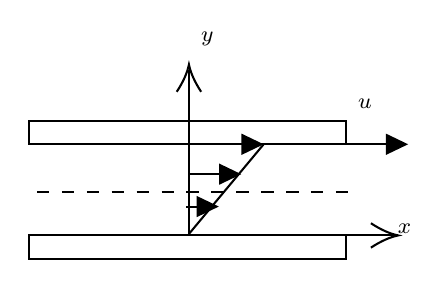
\begin{tikzpicture}[x=0.75pt,y=0.75pt,yscale=-1.2,xscale=1.2]
		%uncomment if require: \path (0,300); %set diagram left start at 0, and has height of 300
		
		%Shape: Rectangle [id:dp6504995050404908] 
		\draw   (68,65) -- (195.33,65) -- (195.33,74.4) -- (68,74.4) -- cycle ;
		%Shape: Rectangle [id:dp7129301360016395] 
		\draw   (68,111) -- (195.33,111) -- (195.33,120.4) -- (68,120.4) -- cycle ;
		%Straight Lines [id:da9429750518588422] 
		\draw    (195.33,74.4) -- (217.33,74.4) ;
		\draw [shift={(220.33,74.4)}, rotate = 180] [fill={rgb, 255:red, 0; green, 0; blue, 0 }  ][line width=0.08]  [draw opacity=0] (8.93,-4.29) -- (0,0) -- (8.93,4.29) -- cycle    ;
		%Straight Lines [id:da44294189343321344] 
		\draw    (132.33,110.4) -- (132.33,44.4) ;
		\draw [shift={(132.33,42.4)}, rotate = 450] [color={rgb, 255:red, 0; green, 0; blue, 0 }  ][line width=0.75]    (10.93,-4.9) .. controls (6.95,-2.3) and (3.31,-0.67) .. (0,0) .. controls (3.31,0.67) and (6.95,2.3) .. (10.93,4.9)   ;
		%Straight Lines [id:da32464864409845406] 
		\draw    (132.33,74.4) -- (159.33,74.4) ;
		\draw [shift={(162.33,74.4)}, rotate = 180] [fill={rgb, 255:red, 0; green, 0; blue, 0 }  ][line width=0.08]  [draw opacity=0] (8.93,-4.29) -- (0,0) -- (8.93,4.29) -- cycle    ;
		%Straight Lines [id:da32461013403386263] 
		\draw    (162.33,74.4) -- (132.33,110.4) ;
		%Straight Lines [id:da6156441304137001] 
		\draw    (132.33,86.4) -- (150.33,86.4) ;
		\draw [shift={(153.33,86.4)}, rotate = 180] [fill={rgb, 255:red, 0; green, 0; blue, 0 }  ][line width=0.08]  [draw opacity=0] (8.93,-4.29) -- (0,0) -- (8.93,4.29) -- cycle    ;
		%Straight Lines [id:da9344339997871164] 
		\draw    (131.33,99.4) -- (141.33,99.4) ;
		\draw [shift={(144.33,99.4)}, rotate = 180] [fill={rgb, 255:red, 0; green, 0; blue, 0 }  ][line width=0.08]  [draw opacity=0] (8.93,-4.29) -- (0,0) -- (8.93,4.29) -- cycle    ;
		%Straight Lines [id:da6156441304137001] 
		\draw    (192.33,111) -- (216.33,111) ;
		\draw [shift={(216.33,111)}, rotate = 180] [color={rgb, 255:red, 0; green, 0; blue, 0 }  ][line width=0.75]    (10.93,-4.9) .. controls (6.95,-2.3) and (3.31,-0.67) .. (0,0) .. controls (3.31,0.67) and (6.95,2.3) .. (10.93,4.9)   ;
		%Straight Lines [id:da8741902353398002] 
		\draw  [dash pattern={on 4.5pt off 4.5pt}]  (71.33,93.4) -- (198.33,93.4) ;
		
		% Text Node
		\draw (136,28) node [anchor=north west][inner sep=0.75pt]  [font=\footnotesize]  {$y$};
		% Text Node
		\draw (215,105) node [anchor=north west][inner sep=0.75pt]  [font=\footnotesize]  {$x$};
		% Text Node
		\draw (199,55) node [anchor=north west][inner sep=0.75pt]  [font=\footnotesize]  {$u$};
	\end{tikzpicture}
\caption{Vertical velocity profile developed in gas between two parallel planes. The top plane moves with velocity $ u $ to the right}
\label{fig:vis-profile}
\end{marginfigure}

At an imaginary plane (e.g. the dashed line in the figure), there must be exchange of molecular momenta as molecules that pass the plane from below have on average slower velocities at $ x- $direction than those pass it from above. \textit{\textbf{Would it be that the viscosity of gas is resulted from such momentum exchange?}} To calculate the net momentum exchange at the imaginary plane, we first need to know \textbf{the average vertical distance $ \bar{y} $ from the imaginary plane where molecules had last collision before they pass the plane}.  As we will see later, $ \bar{y} $ helps us to find the average $ x- $momentum of molecules that pass the imaginary plane.

Based on the terminology we developed in Lab1, the mass flux of molecules arriving at the imaginary plane in a polar angle $ \theta $ is obtained by integrating over azimuthal angle and velocity magnitude in Eq.(\ref{eq:mass-flux}), i.e,
\begin{equation}
	\Phi_{\theta} = \frac{1}{2}n\bar{v}\sin(\theta)\cos(\theta)\Delta \theta.
	\label{eq:Phi-theta}
\end{equation}
The total mass flux is then
\begin{equation}
	\Phi =\int_0^{\pi/2}\Phi_{\theta}d\theta =\frac{1}{4}n\bar{v}.
	\label{eq:Phi-tot}
\end{equation}
Given Eq.(\ref{eq:Phi-theta}) and (\ref{eq:Phi-tot}), the averaged vertical distance $\bar{y}$ is then
\begin{equation}
	\bar{y} = \frac{n\bar{v}\int_0^{\pi/2}\sin(\theta)\cos(\theta)l\cos(\theta)d\theta}{2\Phi}=\frac{2}{3}l,
	\label{eq:bar-y}
\end{equation}
where $ l\cos(\theta) $ is the vertical distance between the imaginary plane and the latest collisions that cause molecules arriving at the plane at a polar angle of $ \theta $ (see Fig.\ref{fig:lcostheta}).
\begin{marginfigure}
	\tikzset{every picture/.style={line width=0.75pt}} %set default line width to 0.75pt        
	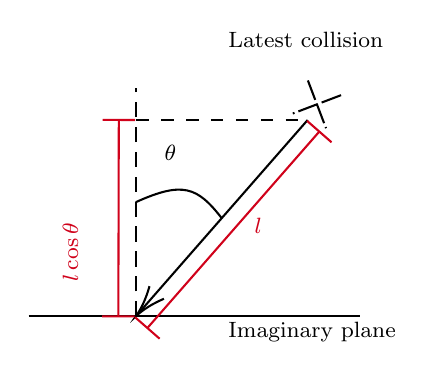
\begin{tikzpicture}[x=0.75pt,y=0.75pt,yscale=-1.4,xscale=1.4]
		%uncomment if require: \path (0,300); %set diagram left start at 0, and has height of 300
		
		%Straight Lines [id:da6518501381186546] 
		\draw    (360.33,166) -- (474.33,166) ;
		%Straight Lines [id:da00009935868456067976] 
		\draw  [dash pattern={on 5.5pt off 3.5pt}]  (397.17,166) -- (397.17,87.4) ;
		%Straight Lines [id:da17820993869324053] 
		\draw    (456.33,98.4) -- (398.48,164.5) ;
		\draw [shift={(397.17,166)}, rotate = 311.19] [color={rgb, 255:red, 0; green, 0; blue, 0 }  ][line width=0.75]    (10.93,-3.29) .. controls (6.95,-1.4) and (3.31,-0.3) .. (0,0) .. controls (3.31,0.3) and (6.95,1.4) .. (10.93,3.29)   ;
		\draw  [dash pattern={on 7.5pt off 1.5pt}] (456.4,84.81) -- (462.64,101.25)(467.82,89.87) -- (451.21,96.18) ;
		%Curve Lines [id:da029089183474892533] 
		\draw    (397.17,126.7) .. controls (413.33,119.4) and (418.33,121.4) .. (426.75,132.2) ;
		%Straight Lines [id:da32957310524805206] 
		\draw [color={rgb, 255:red, 208; green, 2; blue, 27 }  ,draw opacity=1 ]   (401.17,170) -- (460.33,102.4) ;
		\draw [shift={(460.33,102.4)}, rotate = 491.19] [color={rgb, 255:red, 208; green, 2; blue, 27 }  ,draw opacity=1 ][line width=0.75]    (0,5.59) -- (0,-5.59)   ;
		\draw [shift={(401.17,170)}, rotate = 491.19] [color={rgb, 255:red, 208; green, 2; blue, 27 }  ,draw opacity=1 ][line width=0.75]    (0,5.59) -- (0,-5.59)   ;
		%Straight Lines [id:da24542469822084534] 
		\draw  [dash pattern={on 4.5pt off 4.5pt}]  (397.33,98.4) -- (456.33,98.4) ;
		%Straight Lines [id:da43445737065249856] 
		\draw [color={rgb, 255:red, 208; green, 2; blue, 27 }  ,draw opacity=1 ]   (391.17,166) -- (391.33,98.4) ;
		\draw [shift={(391.33,98.4)}, rotate = 450.14] [color={rgb, 255:red, 208; green, 2; blue, 27 }  ,draw opacity=1 ][line width=0.75]    (0,5.59) -- (0,-5.59)   ;
		\draw [shift={(391.17,166)}, rotate = 450.14] [color={rgb, 255:red, 208; green, 2; blue, 27 }  ,draw opacity=1 ][line width=0.75]    (0,5.59) -- (0,-5.59)   ;
		
		% Text Node
		\draw (406,106) node [anchor=north west][inner sep=0.75pt]  [font=\footnotesize]  {$\theta $};
		% Text Node
		\draw (428,67) node [anchor=north west][inner sep=0.75pt]  [font=\footnotesize] [align=left] {Latest collision};
		\draw (428,167) node [anchor=north west][inner sep=0.75pt]  [font=\footnotesize] [align=left] {Imaginary plane};
		% Text Node
		\draw (437,131) node [anchor=north west][inner sep=0.75pt]  [font=\footnotesize,color={rgb, 255:red, 208; green, 2; blue, 27 }  ,opacity=1 ]  {$l$};
		% Text Node
		\draw (371,155) node [anchor=north west][inner sep=0.75pt]  [font=\footnotesize,color={rgb, 255:red, 208; green, 2; blue, 27 }  ,opacity=1 ,rotate=-270]  {$l\cos \theta $};
		
		
	\end{tikzpicture}
\caption{Vertical distance between the imaginary plane and the latest collision}
\label{fig:lcostheta}
\end{marginfigure}

Let $ u_0 $ be the $ x- $velocity at the imaginary plane, then the $ x- $momentum of molecules pass the plane from above is them
\begin{equation}
	p_x^{+}=m(u_0+\frac{2}{3}l\frac{du}{dy}),
	\label{eq:px+}
\end{equation}
according to Taylor expansion. Similarly, for those below the plane, their $ x- $momentum is simply
\begin{equation}
	p_x^{-}=m(u_0-\frac{2}{3}l\frac{du}{dy}),
	\label{eq:px-}
\end{equation}
and the change in $ x- $momentum from the "fast" to the "slow" is 
\begin{equation}
	\Delta p_x = m\frac{4}{3}l\frac{du}{dy}.\label{eq:dp-x}
\end{equation}
Multiplying both sides of Eq.(\ref{eq:dp-x}) by the $\Phi$ in Eq.(\ref{eq:Phi-tot}) gives the "viscous force" per unit area at the LHS\footnote{we used this trick before in Lab1}, i.e.,
\begin{equation}
	\frac{F_{vis}}{A} = \frac{4}{3}ml\Phi\frac{du}{dy}.
\end{equation}
Since the viscosity coefficient $ \eta $ is defined through the equation 
\begin{equation}
	\frac{F_{vis}}{A} = \eta\frac{du}{dy},
	\label{eq:viscosity}
\end{equation}
we finally obtain an explicit expression for $ \eta $ as
\begin{equation}
	\eta = \frac{m\bar{v}}{3\sigma}.
	\label{eq:eta}
\end{equation}
Eq.(\ref{eq:eta}) is very interesting as it indicates that the viscosity of gas does not depend on gas density but average molecular velocity. With the method developed here, deriving an expression for thermal conductivity coefficient $ \kappa $ becomes fairly easy.
\subsection{Thermal conductivity from energy transport}
We first notice that Fourier's law looks a lot like Eq.(\ref{eq:viscosity}). Instead of having viscous force per unit area at LHS, we have, in Fourier's law, the heat flux $ q $ proportional to temperature gradient, i.e.,
\begin{equation}
	q = -\kappa\frac{dT}{dy}.
	\label{eq:fourier}
\end{equation}
We again imagine an imaginary plane in the gas, at which the temperature is $ T_0 $. The energy of single molecule at the plane is $ c_v^{\prime}T_0 $ with $ c_v^{\prime} $ being the "specific heat" per molecule. By following the formalism in Eq. (\ref{eq:px+}) and (\ref{eq:px-}), the molecular energies above and below the plane before their arrival are
\begin{equation}
	E_{above} = c_v^{\prime}(T_0+\frac{2}{3}l\frac{dT}{dy})
\end{equation}
and
\begin{equation}
	E_{below} = c_v^{\prime}(T_0-\frac{2}{3}l\frac{dT}{dy}).
\end{equation}
Following the same logic laid out in the previous subsection\footnote{Notice that $ dT/dy $ is negative here, so $ E_{below}-E_{above}>0 $}, we have
\begin{equation}
	\Phi\times(E_{below}-E_{above}) = -\frac{c_v^{\prime}\bar{v}}{3\sigma}\frac{dT}{dy} = -\kappa\frac{dT}{dy},
\end{equation}
and
\begin{equation}
	\kappa = \frac{c_v^{\prime}\bar{v}}{3\sigma}.
	\label{eq:kappa}
\end{equation}
From Eq.(\ref{eq:kappa}), we find that the thermal conductivity of gas is inversely proportional to the size of molecule. The gas molecule that can move fast and store lots of thermal energy tends to have better thermal conductivity.
\section{Inadequacy of hard-sphere assumption}
Based on our derivation of $ \eta $ and $ \kappa $, the ratio of the two gives
\begin{equation}
	\kappa/\eta = \frac{c_v^{\prime}}{m} = \frac{c_v}{M}
\end{equation} 
where $ c_v $ and $ M $ are the specific heat and the molar mass of gas molecule, respectively. From this, we have
 \begin{equation}
 	\frac{\eta c_v}{\kappa M}=1.
 	\label{eq:unity-eta-kapp}
 \end{equation} 

Everything in Eq.(\ref{eq:unity-eta-kapp}) is experimentally measurable, so we can test this relationship on real gases. However, real gases usually have such value around $ 0.5 $, not $ 1 $\footnote{For air, the ratio has a value of 0.51546.}, which means our hard-sphere assumption does not capture the whole story of molecular collisions. But at least it got the order of magnitude right. To make the assumption more realistic, we might have no choice but to consider what is happening at the moment of molecular collision, an interesting realm for chemists, physicists, and me.